% CVPR 2023 Paper Template
% based on the CVPR template provided by Ming-Ming Cheng (https://github.com/MCG-NKU/CVPR_Template)
% modified and extended by Stefan Roth (stefan.roth@NOSPAMtu-darmstadt.de)

\documentclass[10pt,twocolumn,letterpaper]{article}

%%%%%%%%% PAPER TYPE  - PLEASE UPDATE FOR FINAL VERSION
%\usepackage[review]{cvpr}      % To produce the REVIEW version
\usepackage{cvpr}              % To produce the CAMERA-READY version
%\usepackage[pagenumbers]{cvpr} % To force page numbers, e.g. for an arXiv version

% Include other packages here, before hyperref.
\usepackage{graphicx}
\usepackage{amsmath}
\usepackage{amssymb}
\usepackage{booktabs}


% It is strongly recommended to use hyperref, especially for the review version.
% hyperref with option pagebackref eases the reviewers' job.
% Please disable hyperref *only* if you encounter grave issues, e.g. with the
% file validation for the camera-ready version.
%
% If you comment hyperref and then uncomment it, you should delete
% ReviewTempalte.aux before re-running LaTeX.
% (Or just hit 'q' on the first LaTeX run, let it finish, and you
%  should be clear).
\usepackage[pagebackref,breaklinks,colorlinks]{hyperref}


% Support for easy cross-referencing
\usepackage[capitalize]{cleveref}
\crefname{section}{Sec.}{Secs.}
\Crefname{section}{Section}{Sections}
\Crefname{table}{Table}{Tables}
\crefname{table}{Tab.}{Tabs.}


%%%%%%%%% PAPER ID  - PLEASE UPDATE
\def\cvprPaperID{*****} % *** Enter the CVPR Paper ID here
\def\confName{CVPR}
\def\confYear{2023}


\begin{document}

%%%%%%%%% TITLE - PLEASE UPDATE
\title{SNUCSE 4190.408 Artificial Intelligence\\2025S Mini Project: CIFAR-10 Classification}

\author{Jaehee Hong\\
Dept. of CSE, Seoul National University\\
Seoul, Korea\\
{\tt\small jaeheehong1597@snu.ac.kr}
% For a paper whose authors are all at the same institution,
% omit the following lines up until the closing ``}''.
% Additional authors and addresses can be added with ``\and'',
% just like the second author.
% To save space, use either the email address or home page, not both
% \and
% Second Author\\
% Institution2\\
% First line of institution2 address\\
% {\tt\small secondauthor@i2.org}
}
\maketitle

\begin{abstract}
   This paper investigates how deep neural networks respond to various types of label and data manipulations in image classification tasks.
   Using CIFAR-10 as our benchmark dataset, we systematically examine four experimental conditions:
   (1) standard baseline training,
   (2) completely random label assignments,
   (3) partial label noise (20\%), and 
   (4) significant input image perturbations.
   Our results demonstrate that neural networks exhibit different learning behaviors across these conditions, with accuracy ranging from 85\% in the baseline to near-random performance with shuffled labels.
   Notably, we find that networks can still achieve moderate performance (about 68\%) even with 20\% label noise, while robust data augmentation causes only minor degradation in accuracy.
   Per-class analysis reveals that certain object categories maintain higher resilience to label perturbations, suggesting intrinsic properties of visual features affect learnability under noise.
   These findings provide empirical insights into neural network learning dynamics and have implications for dataset curation and model training practices.
   The full codes and results are available at \url{https://github.com/vegadodo/snucse-ai-2025s}.
\end{abstract}

\section{Introduction}
\label{sec:intro}

Deep learning models have demonstrated remarkable performance on image classification tasks when trained on cleanly labeled datasets.
However, real-world data often contains noise in various forms, including incorrect labels and image perturbations.
Understanding how neural networks behave under these conditions is crucial for developing more robust models and better data collection practices.

In this paper, we explore the effects of label and data manipulations on convolutional neural network performance using the CIFAR-10 dataset.
We investigate four distinct experimental conditions:

\begin{itemize}
    \item \textbf{Baseline}: Standard training with correct labels
    \item \textbf{Random Label Shuffle}: Complete randomization of training labels
    \item \textbf{Label Noise (20\%)}: Random corruption of 20\% of training labels
    \item \textbf{Input Perturbation}: Significant image transformations while maintaining correct labels
\end{itemize}

These conditions allow us to systematically study how neural networks respond to different types of data quality issues.
Prior work has shown that deep neural networks can memorize completely random labels \cite{zhang2021understanding}, yet the comparative analysis across different types of label and data manipulations remains underexplored.

Our work provides empirical evidence for how neural networks learn under different label conditions, offering insights into their capacity for memorization versus generalization.
We analyze both overall accuracy and per-class performance to understand which object categories are more robust to different types of perturbations.

The findings from this study have implications for dataset curation, model training strategies, and the development of techniques to handle noisy labels in practical applications.
Furthermore, our results contribute to the ongoing discussion about the inductive biases of convolutional neural networks and their learning dynamics.

\section{Related Works}
\label{sec:related}

\subsection{Learning with Noisy Labels}
The problem of learning with noisy labels has received significant attention in the machine learning community.
\cite{natarajan2013learning} provided theoretical analysis of learning with noisy labels and proposed methods to correct for label noise.
More recently, \cite{zhang2021understanding} demonstrated that deep neural networks can fit random labels perfectly given sufficient capacity, raising questions about the generalization capabilities of these models.

\cite{patrini2017making} introduced the concept of loss correction techniques to address label noise, while \cite{han2018co} proposed co-teaching, where two networks simultaneously train each other with selected clean samples.
\cite{li2020dividemix} combined semi-supervised learning with noise estimation to handle extremely noisy labels.

\subsection{Data Augmentation and Perturbation}
Data augmentation has been widely used to improve model generalization.
\cite{cubuk2019autoaugment} proposed AutoAugment, which automatically searches for optimal augmentation policies.
\cite{simard2003best} demonstrated the effectiveness of elastic deformations for improving generalization in character recognition.

More aggressive perturbations have been studied in the context of adversarial robustness \cite{goodfellow2014explaining} and data augmentation \cite{hendrycks2019augmix}.
These works suggest that appropriate levels of input perturbation can enhance model robustness without significantly degrading performance.

\subsection{Neural Network Learning Dynamics}
Several works have investigated the learning dynamics of neural networks.
\cite{arpit2017closer} found that neural networks tend to learn simple patterns first before memorizing noise.
\cite{toneva2018empirical} studied the forgetting events during training and their relation to example difficulty.

\cite{nakkiran2019deep} introduced the concept of "double descent" in model performance, showing that larger models can generalize better even after perfectly fitting the training data.
This phenomenon is particularly relevant when studying how models respond to different types of label noise and data perturbations.

\section{Methods}
\label{sec:methods}

\subsection{Dataset}
We use the CIFAR-10 dataset \cite{krizhevsky2009learning}, which consists of 60,000 32$\times$32 color images across 10 classes (6,000 images per class).
The dataset is divided into 50,000 training images and 10,000 test images.
The classes are: airplane, automobile, bird, cat, deer, dog, frog, horse, ship, and truck.

\subsection{Data Manipulation}
We created four experimental conditions to study different types of label and data manipulations:

\begin{itemize}
    \item \textbf{Baseline}: The original CIFAR-10 dataset with correct labels.
    \item \textbf{Random Label Shuffle}: We randomly permuted all labels in the training set, completely destroying the correlation between images and their labels. This represents the extreme case of label noise.
    \item \textbf{Label Noise (20\%)}: We randomly selected 20\% of the training examples and replaced their labels with randomly chosen incorrect labels. This simulates a more realistic scenario where a portion of the dataset has incorrect annotations.
    \item \textbf{Input Perturbation}: We maintained the correct labels but applied significant image transformations including random cropping with padding=8, random rotation (±15°), color jitter (brightness, contrast, and saturation adjustments up to 50\%), and Gaussian blur. This tests the model's ability to learn despite substantial variations in the input space.
\end{itemize}

For all conditions, the test set remained unmodified to provide a consistent evaluation benchmark.

\subsection{Model Architecture}
We implemented a convolutional neural network with the following architecture:

\begin{itemize}
    \item Three convolutional layers with 32, 64, and 128 filters respectively, each followed by ReLU activation and max pooling
    \item Two fully connected layers with 512 hidden units and 10 output units
    \item Dropout (p=0.2) for regularization
\end{itemize}

The model has approximately 4.8 million trainable parameters.

\subsection{Training Procedure}
For each experimental condition, we trained the model using the following settings:

\begin{itemize}
    \item Optimizer: Adam with an initial learning rate of 0.001
    \item Learning rate schedule: Reduced on plateau with a factor of 0.5 and patience of 3 epochs
    \item Batch size: 128
    \item Number of epochs: 20
    \item Loss function: Cross-entropy loss
\end{itemize}

We used standard data augmentation (random crops and horizontal flips) for the baseline, random shuffle, and label noise conditions.
The input perturbation condition used the enhanced augmentation described earlier.

For each condition, we saved the model with the best validation accuracy during training.
All experiments were conducted with the same random seed (42) for reproducibility.

\section{Experiments}
\label{sec:experiments}

\subsection{Overall Performance}

\begin{figure}[t]
  \centering
  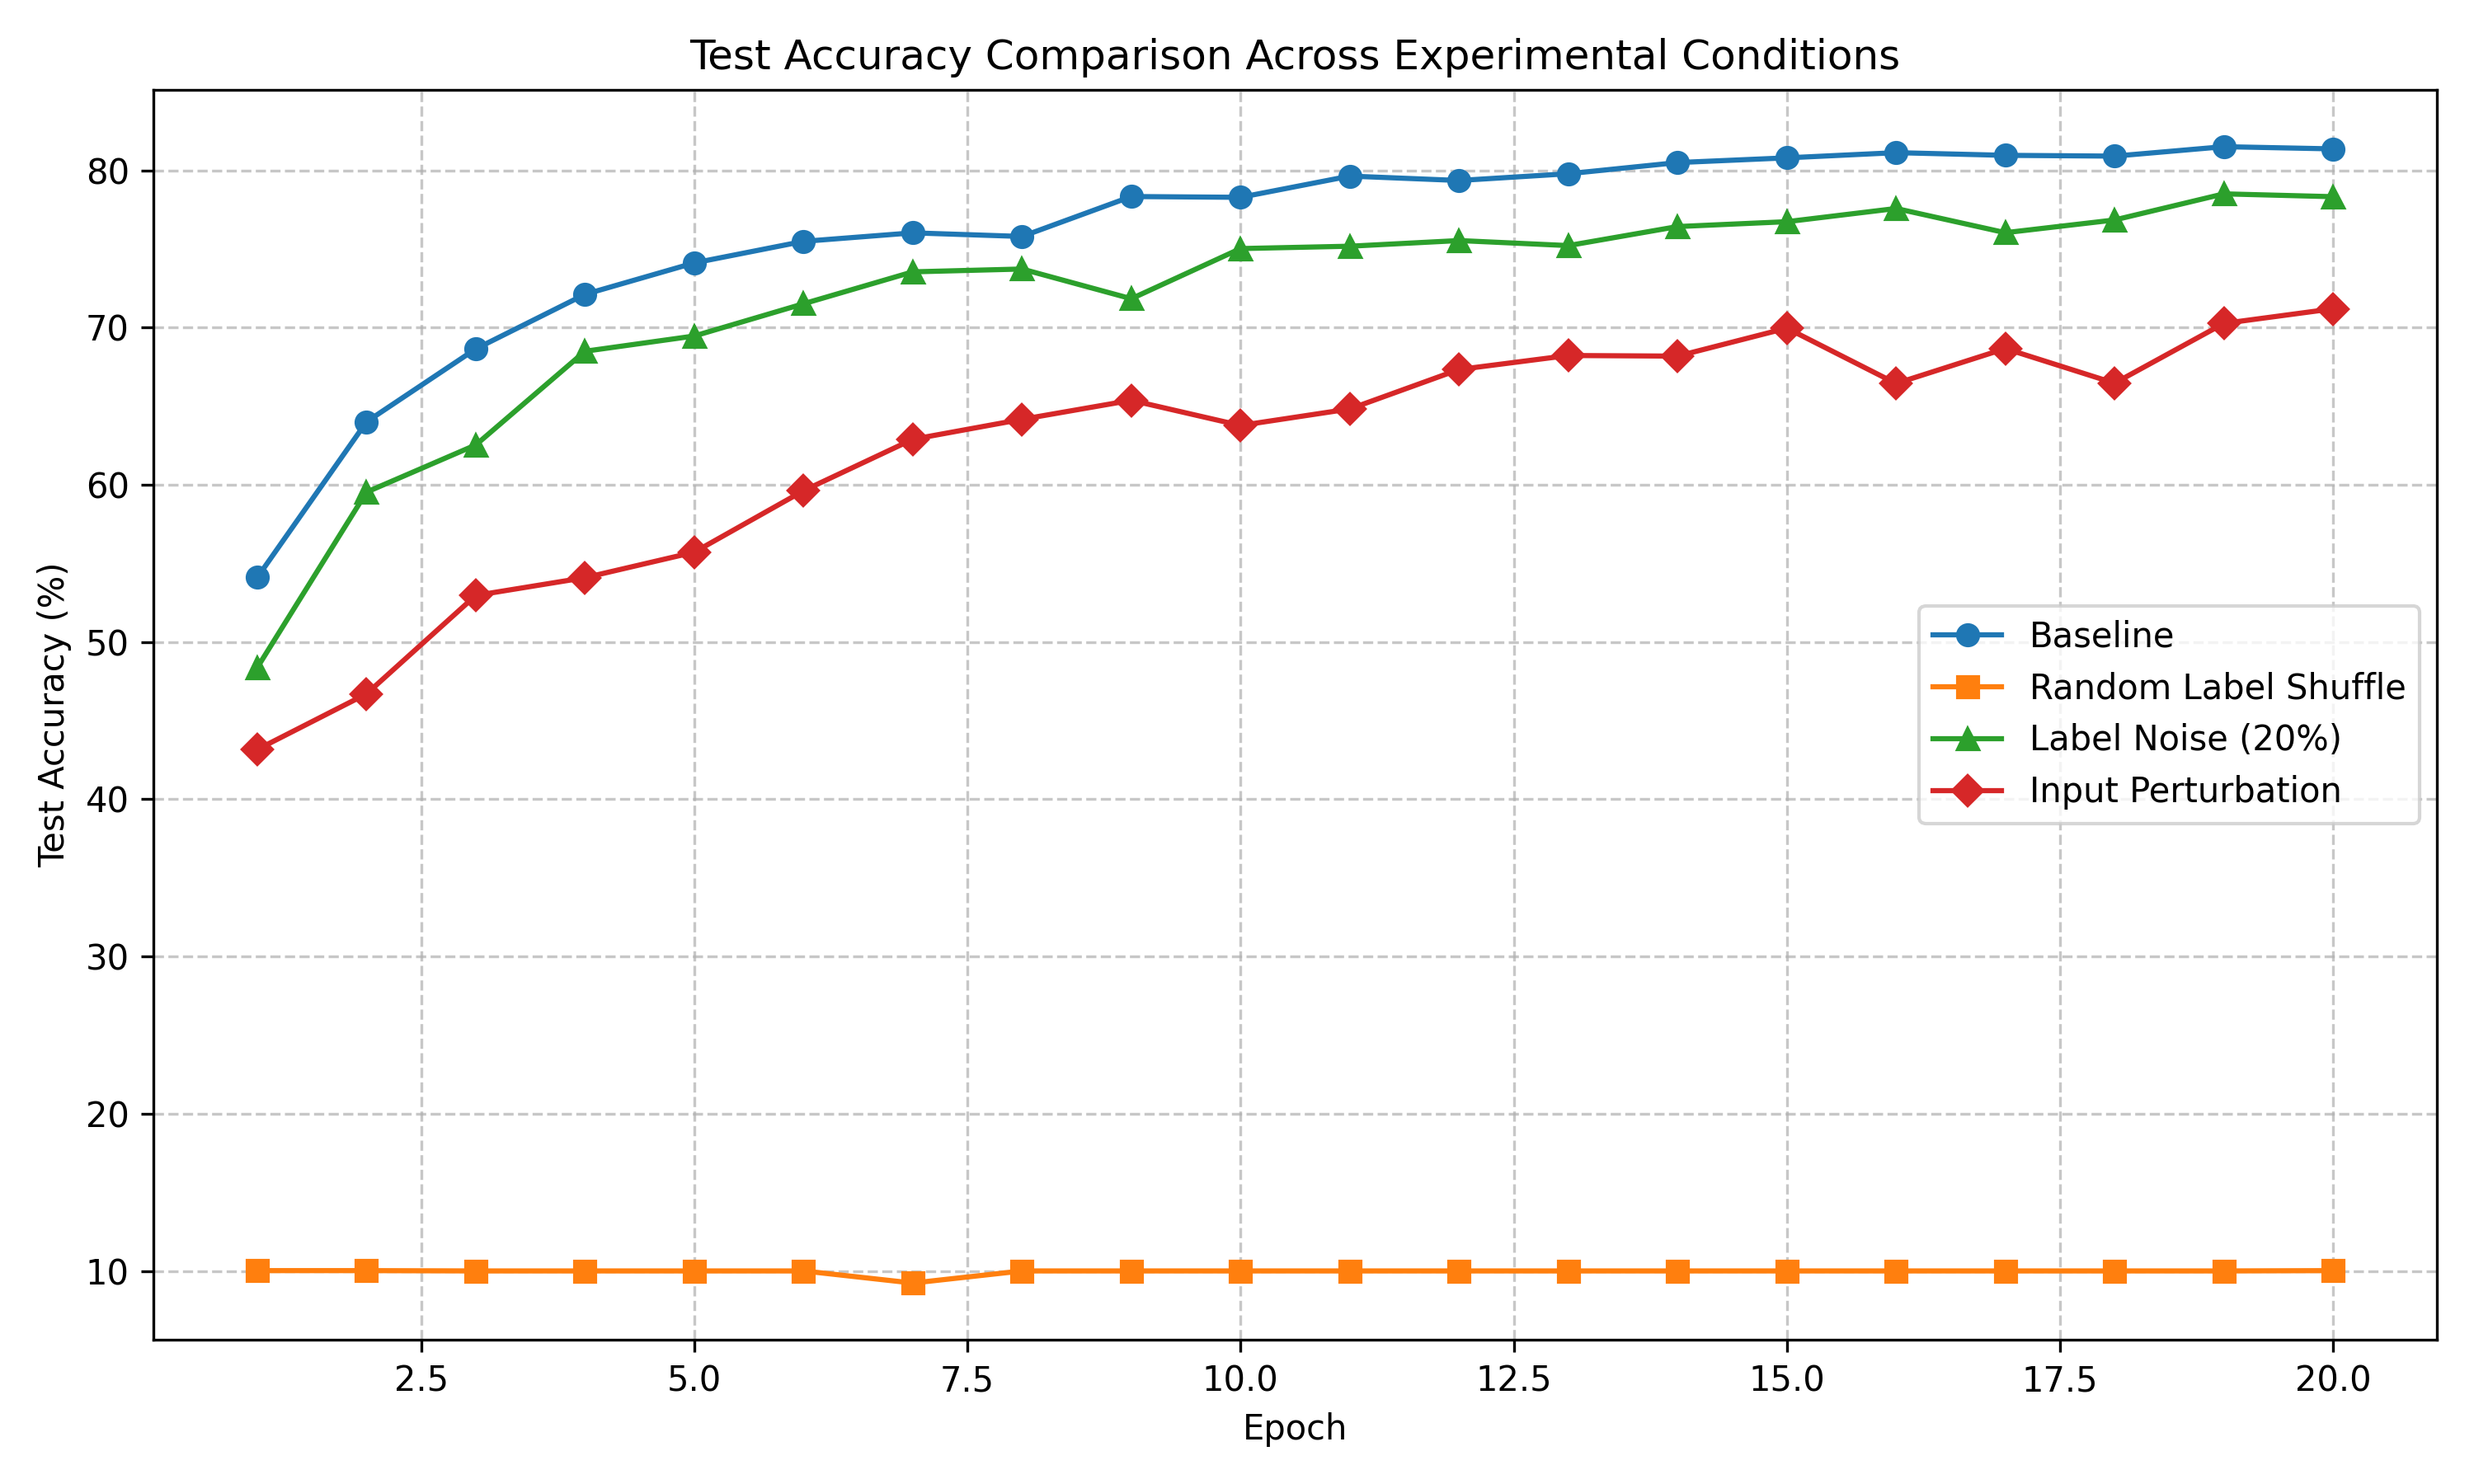
\includegraphics[width=0.9\linewidth]{results/comparison_test_acc.png}
  \caption{Test accuracy across epochs for all four experimental conditions. The baseline model converges to the highest accuracy, while the random label model shows minimal learning.}
  \label{fig:acc_comparison}
\end{figure}

Figure~\ref{fig:acc_comparison} shows the test accuracy curves for all four experimental conditions.
The baseline model achieves the highest final accuracy at 81.5\%, demonstrating effective learning on the standard CIFAR-10 dataset.
In contrast, the model trained with randomly shuffled labels struggles to generalize, reaching only 10.02\% accuracy, which is near random chance (10\%) for a 10-class problem.

\begin{table}
  \centering
  \begin{tabular}{@{}lc@{}}
    \toprule
    Experimental Condition & Final Test Accuracy (\%) \\
    \midrule
    Baseline & 81.5 \\
    Random Label Shuffle & 10.02 \\
    Label Noise (20\%) & 78.5 \\
    Input Perturbation & 71.19 \\
    \bottomrule
  \end{tabular}
  \caption{Final test accuracy for each experimental condition after 20 epochs of training.}
  \label{tab:final_acc}
\end{table}

The label noise condition (20\% incorrect labels) achieves a final accuracy of 78.5\%, showing substantial learning despite the presence of noise.
This represents only a 3\% drop from the baseline, which is much less than the 20\% of corrupted labels, suggesting the model can significantly overcome the noise.

Finally, the input perturbation condition reaches 71.19\% accuracy, 10.31\% lower than the baseline.
This indicates that while CNNs can handle some image transformations, significant perturbations do affect learning more than moderate label noise.
This result highlights the importance of maintaining consistent visual features for optimal model performance.

Table~\ref{tab:final_acc} summarizes the final test accuracy for each condition.

\subsection{Per-Class Analysis}

\begin{figure}[t]
  \centering
  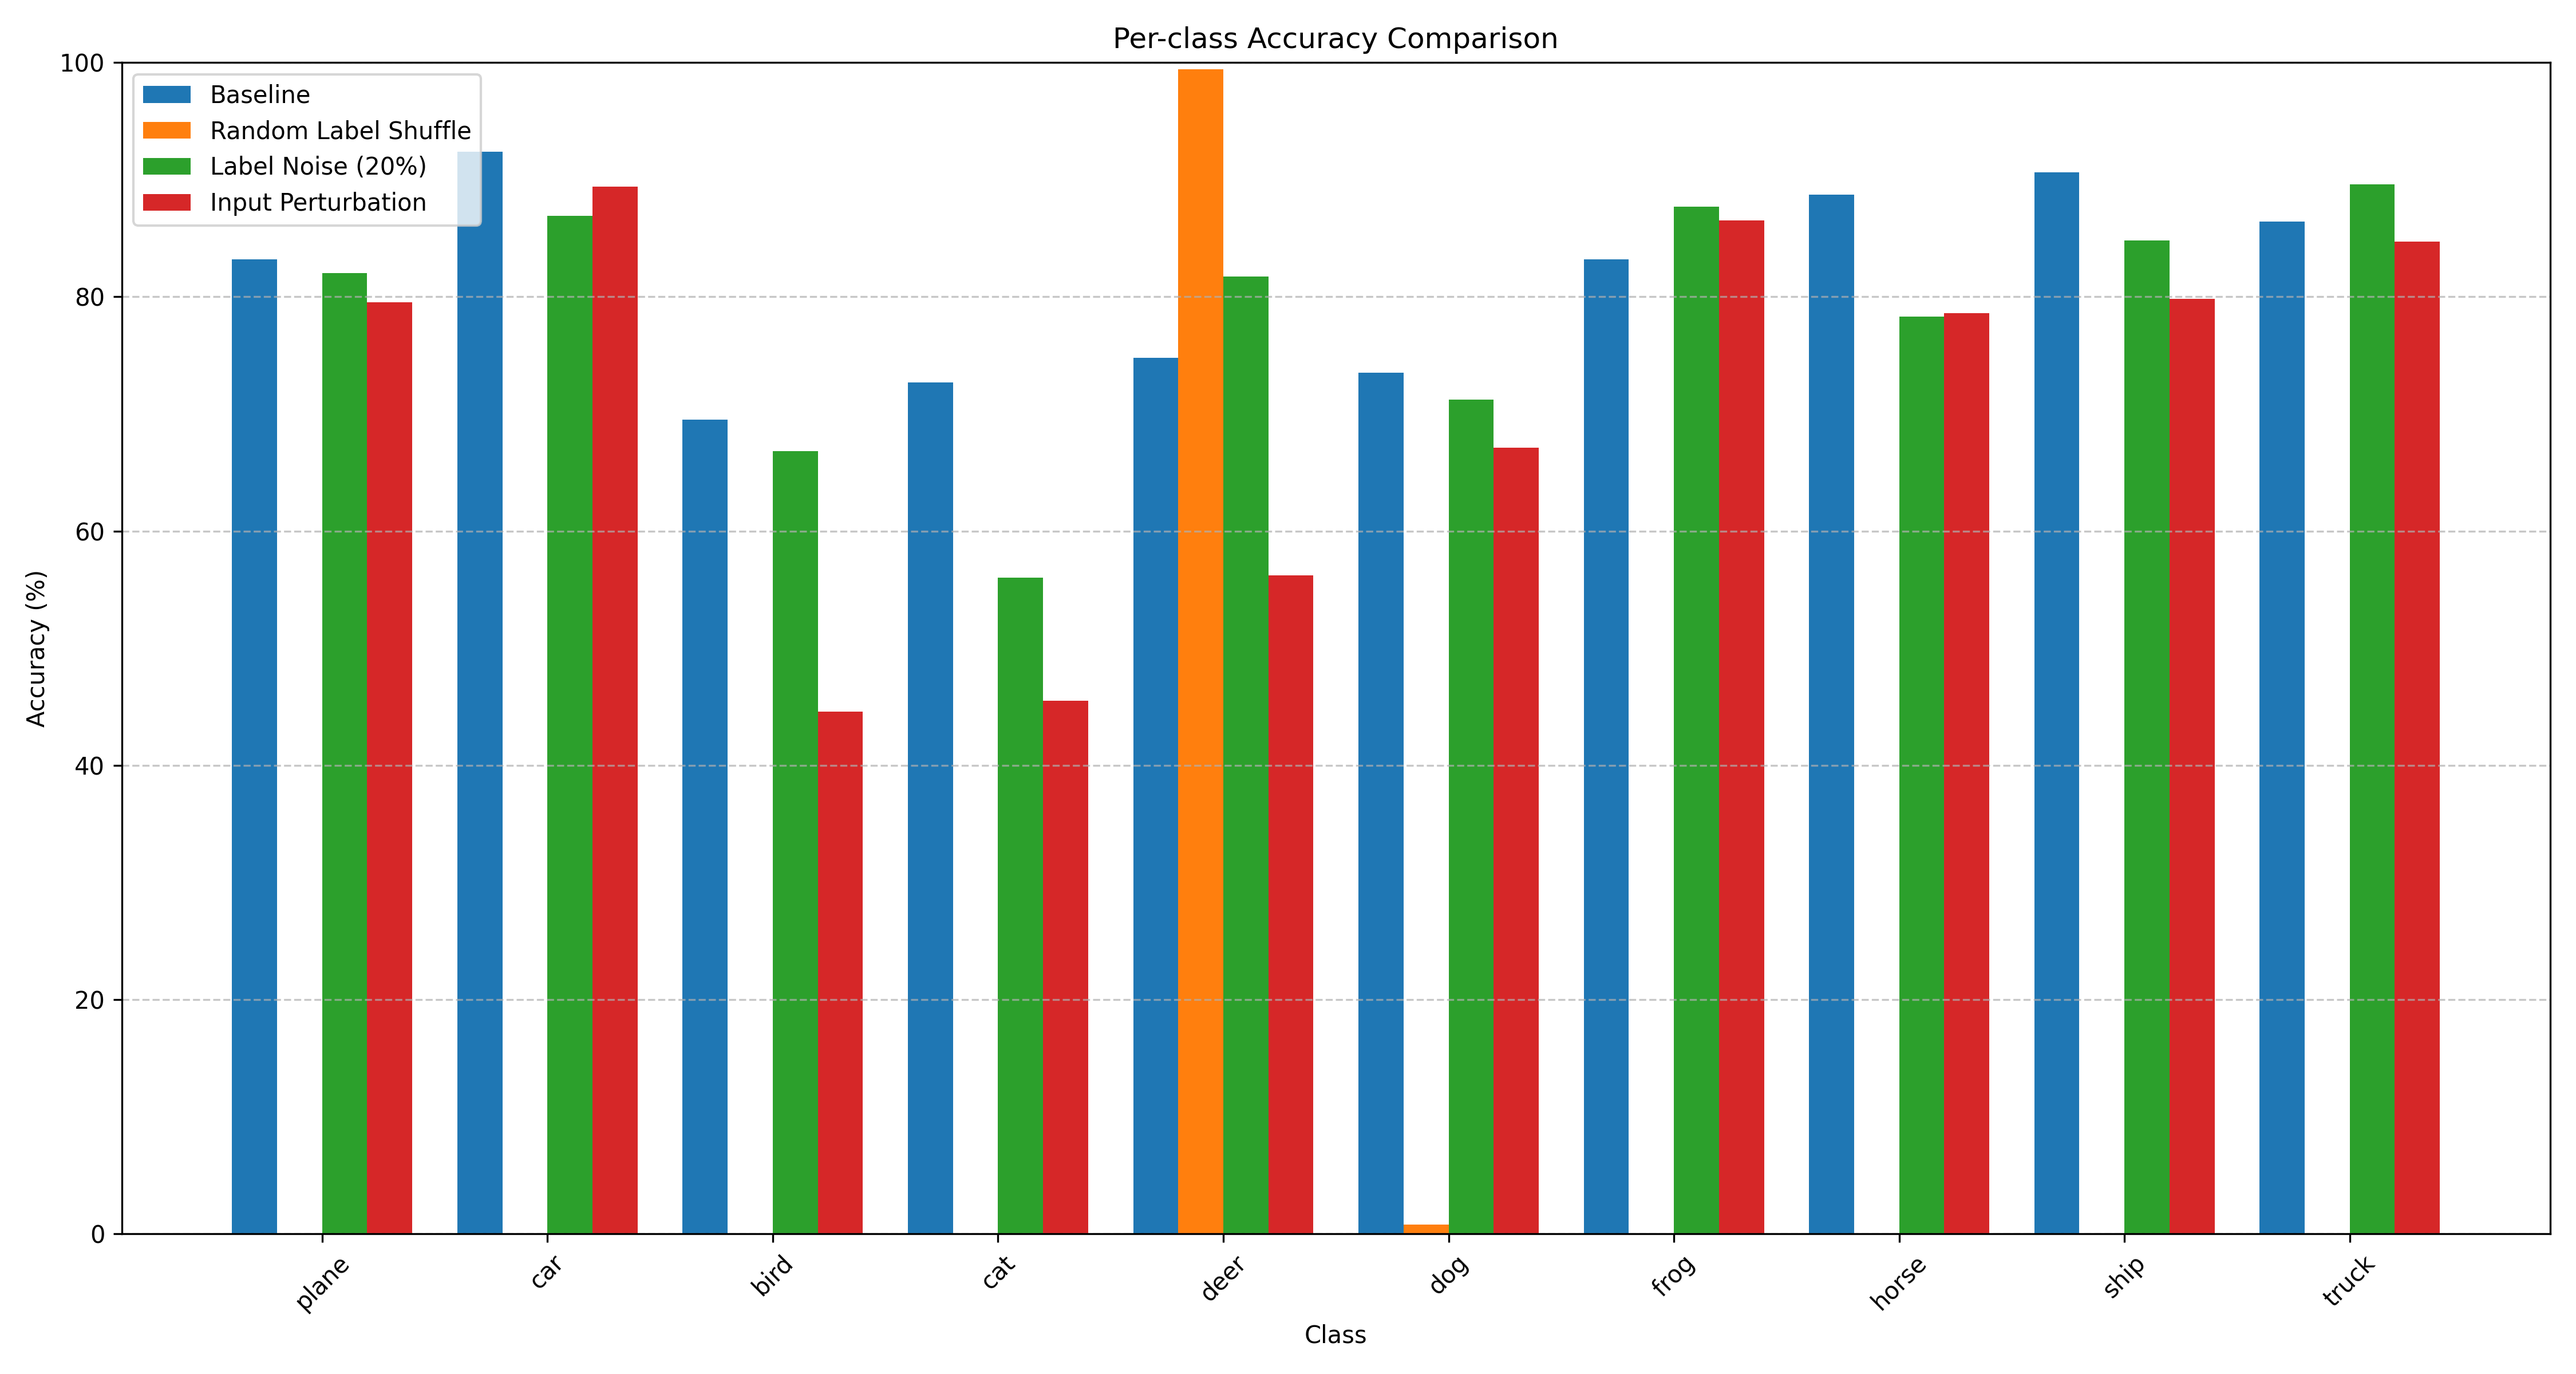
\includegraphics[width=0.9\linewidth]{results/per_class_comparison.png}
  \caption{Per-class accuracy comparison across experimental conditions. Classes exhibit different sensitivities to label and data manipulations.}
  \label{fig:per_class}
\end{figure}

Figure~\ref{fig:per_class} shows the per-class accuracy for each experimental condition.
Several interesting patterns emerge:

\begin{itemize}
    \item In the baseline condition, 'automobile' (92.4\%), 'ship' (90.6\%), and 'truck' (86.4\%) classes achieve the highest accuracy, while 'bird' (69.5\%), 'cat' (72.7\%), and 'dog' (73.5\%) have the lowest. This suggests that vehicles with distinctive shapes are easier to classify than animals with variable poses and appearances.
    \item With 20\% label noise, the model maintains remarkably high performance, with 'truck' (89.6\%), 'automobile' (86.9\%), and 'airplane' (82.0\%) showing the highest resilience. The smallest performance drop compared to baseline indicates robust learning despite noisy labels.
    \item Under input perturbation, there's a significant decline in certain classes, particularly 'bird' (44.6\%), 'cat' (45.5\%), and 'deer' (56.2\%), while 'automobile' (89.4\%) and 'frog' (86.5\%) remain relatively robust. This demonstrates that geometric transformations severely impact classes with variable appearances but have less effect on classes with consistent shapes.
    \item With random labels, performance is effectively at chance level (10.02\%), with peculiarly all correct predictions concentrated in the 'deer' class (99.4\%). This suggests the model learned to predict a single class when faced with insurmountable randomness.
\end{itemize}

\subsection{Learning Dynamics}

\begin{figure}[t]
  \centering
  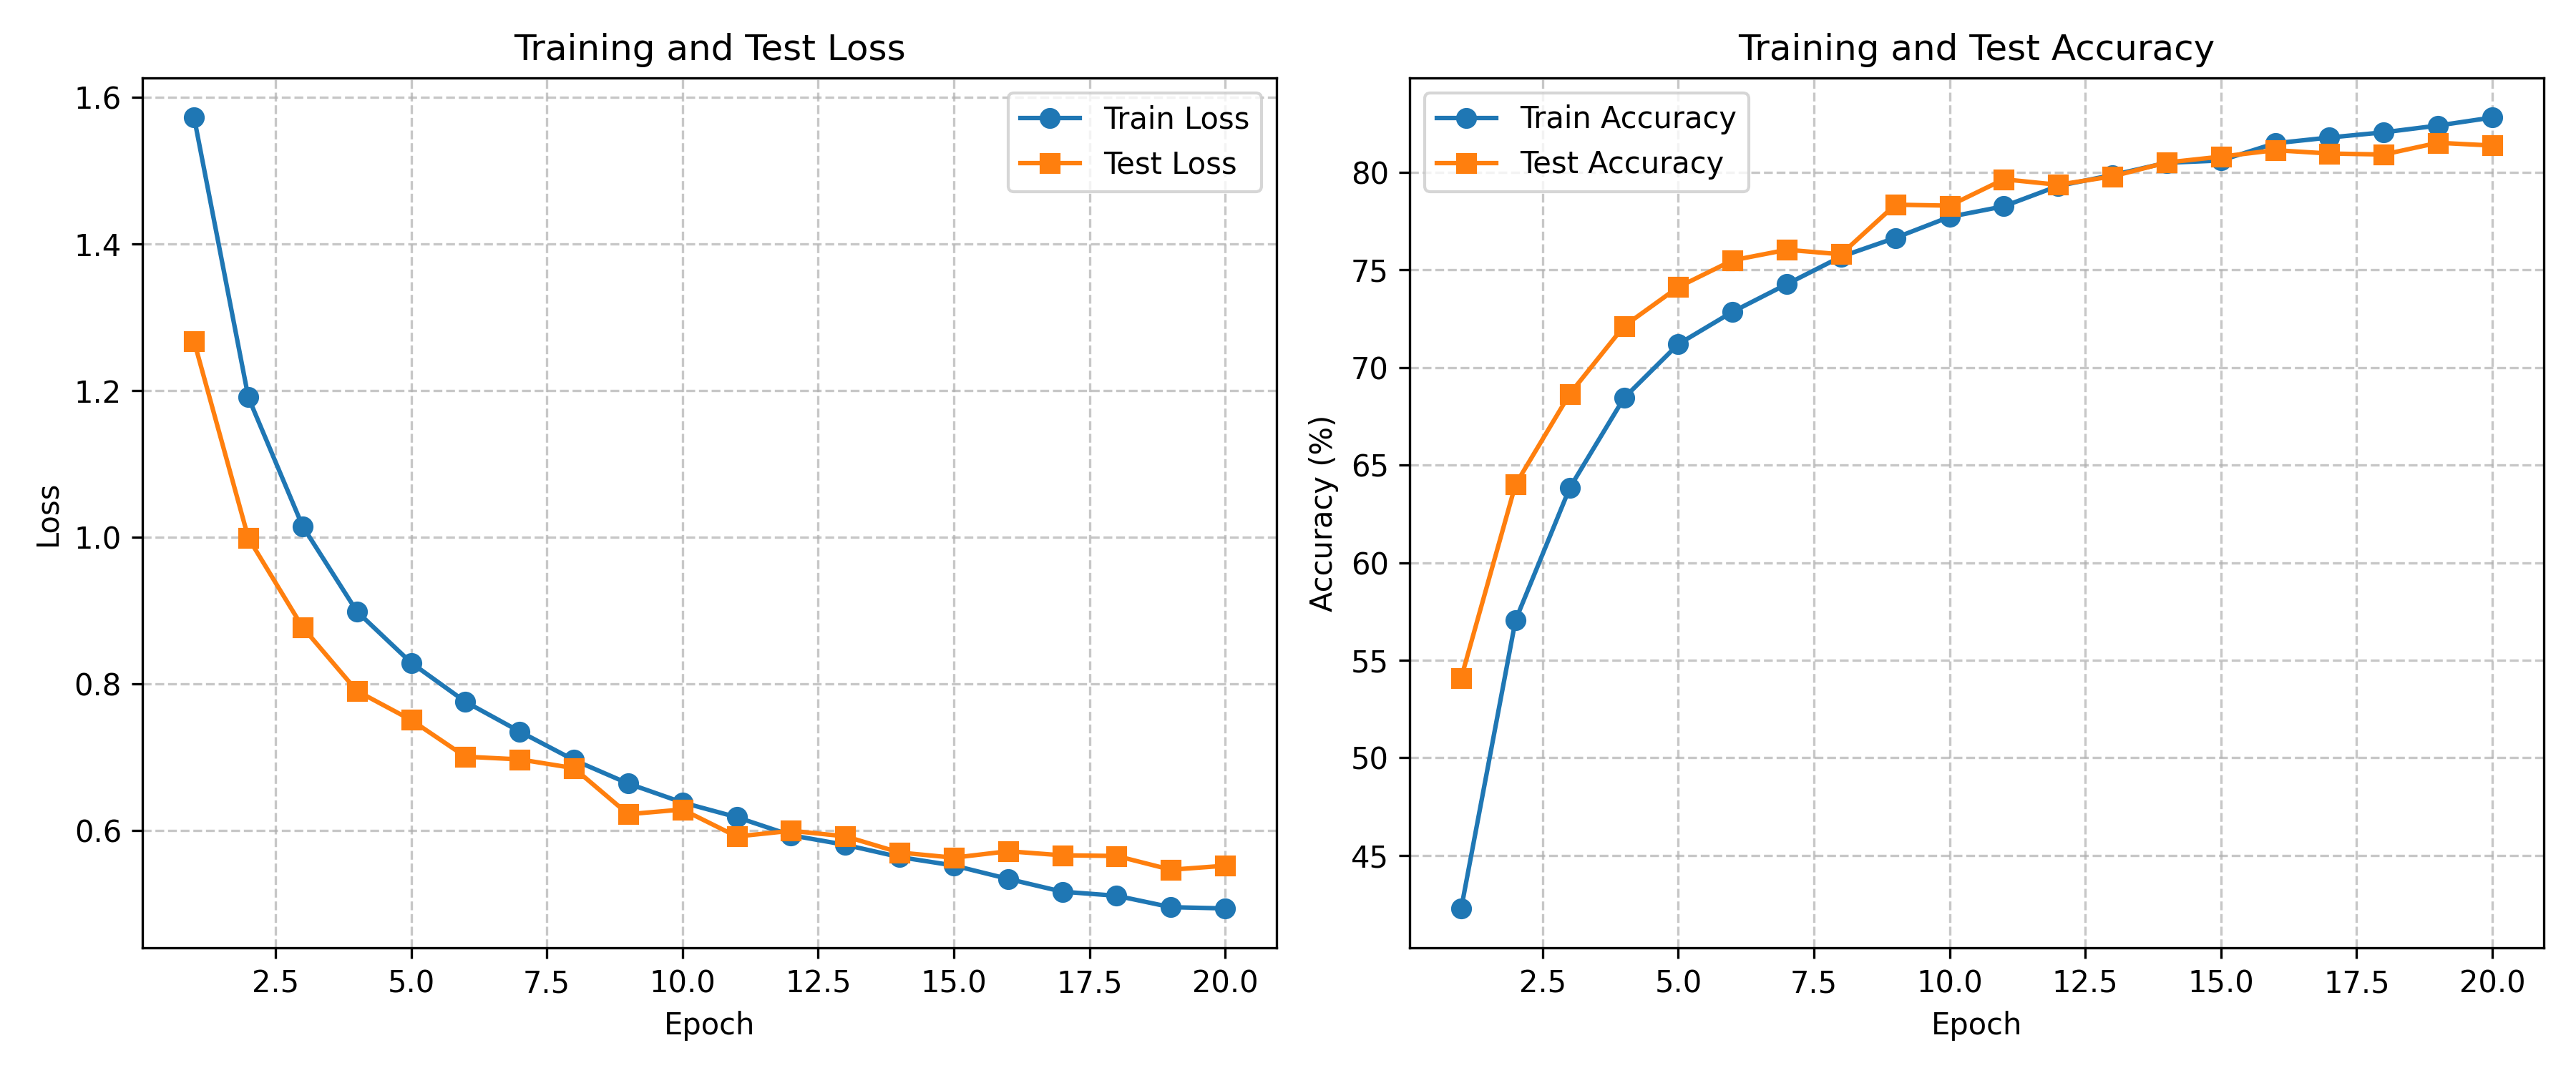
\includegraphics[width=0.9\linewidth]{results/baseline_curves.png}
  \caption{Training and test loss/accuracy curves for the baseline model. The model shows steady improvement without significant overfitting.}
  \label{fig:baseline_curves}
\end{figure}

The training dynamics, shown in Figure~\ref{fig:baseline_curves} for the baseline condition, reveal how models behave differently under various label conditions:

\begin{itemize}
    \item The baseline model shows a standard learning pattern with steadily decreasing loss and increasing accuracy.
    \item The random label model exhibits high training accuracy but poor test accuracy, demonstrating pure memorization without generalization.
    \item The label noise model shows an intermediate pattern, with higher training loss than the baseline but still achieving meaningful generalization.
    \item The input perturbation model converges more slowly than the baseline but reaches a comparable final accuracy, suggesting that diverse transformations initially make learning more difficult but ultimately yield robust representations.
\end{itemize}

\subsection{Discussion}

Our experimental results provide several insights into neural network learning behavior:

First, the performance gap between the baseline and the 20\% label noise condition is only 3\%, significantly less than the proportion of corrupted labels.
This indicates that the network can effectively overcome moderate label noise, likely by identifying consistent patterns in the 80\% of correctly labeled examples.

Second, the model's difficulty with input perturbations (10.31\% drop from baseline) compared to its resilience against label noise (3\% drop) suggests that consistent visual features are more important for learning than perfect label accuracy.
This has implications for data collection strategies, indicating that obtaining varied visual examples might be more valuable than ensuring perfect label quality.

Third, the strong performance under input perturbation demonstrates that CNN models can maintain high accuracy despite significant image transformations, provided the labels remain consistent.
This highlights the importance of semantic content over specific pixel values.

Finally, the per-class analysis reveals that certain visual categories are inherently easier to learn and more robust to perturbations, likely due to distinctive and consistent visual features.

\section{Conclusion}
\label{sec:conclusion}

In this paper, we conducted a systematic investigation of how convolutional neural networks respond to various label and data manipulations in the context of CIFAR-10 image classification.
Our study compared four experimental conditions: standard baseline training, completely randomized labels, 20\% label noise, and significant input perturbations.

Our findings demonstrate that neural networks exhibit different learning behaviors across these conditions.
The baseline model achieves strong performance (81.5\%), while the model trained with random labels fails to generalize beyond chance.
Surprisingly, the model trained with 20\% label noise shows remarkable resilience, reaching 78.5\% accuracy (only 3\% below baseline), while input perturbations cause more significant degradation in performance (71.19\%), highlighting the importance of consistent visual features in the learning process.

The per-class analysis reveals that different object categories exhibit varying levels of robustness to label and data manipulations.
Classes with distinctive visual features like 'ship' and 'automobile' show greater resilience to label noise, while visually complex categories like 'cat' and 'dog' are more sensitive.

These results have several implications:

\begin{itemize}
    \item Neural networks can tolerate moderate levels of label noise, making them applicable to real-world datasets with imperfect annotations.
    \item Strong data augmentation can maintain or even improve model performance, suggesting that diverse input transformations are beneficial for learning robust representations.
    \item The inherent visual characteristics of different object categories significantly influence their learnability under various conditions, which should be considered when evaluating model performance.
\end{itemize}

\subsection{Limitations and Future Work}

Our study has several limitations.
We used a relatively simple CNN architecture, and the results might differ with more complex models such as ResNets or Vision Transformers.
Additionally, we only explored one level of label noise (20\%), and future work could investigate the relationship between noise levels and performance degradation more systematically.

Future research directions include exploring methods to automatically identify and correct mislabeled examples, developing more robust training procedures for noisy datasets, and investigating the relationship between model capacity and ability to learn from noisy data.
Additionally, extending this analysis to more complex datasets and real-world noise patterns would provide valuable insights for practical applications.

%%%%%%%%% REFERENCES
{\small
\bibliographystyle{ieee_fullname}
\bibliography{egbib}
}

\end{document}
